\subsection*{REBEL}
We have built a simple knowledge graph for one instance of a long document.
Specifically, we built a knowledge graph for the first row of the GovReport
validation set. We did this by using an open-source, pre-trained, end-to-end
relation extraction model called REBEL
\cite{huguet2021rebel} which can be found on Hugging
Face here.\footnote{https://huggingface.co/Babelscape/rebel-large} This model
takes an input string and extracts head-relation-tail triplets. A sample of
extracted relations is shown below (see figure \ref{fig-triplets}).

 \begin{figure}[htp]
    \centering
    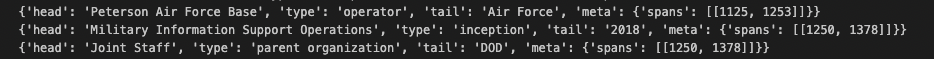
\includegraphics[width=17cm]{images/relations_example.png}
    \caption{Three example triplets extracted from REBEL.}
    \label{fig-triplets}
\end{figure}

We chose to use REBEL because it finds entities and relations at the same time
(end-to-end), it is open source, and it is easy to implement using Hugging
Face. One downside of REBEL is that it is limited in the number of relations
that it can extract (approximately 200).   As a result, we are still looking
into alternatives. Since the pre-trained REBEL model has a token limit, we
wrote some code that splits the long document into 128-token chunks. Triplets
were then extracted for each chunk. Next, we used NetworkX to assemble the
head-relation-tail triplets into a directed graph to form the knowledge graph.
The plotted knowledge graph for the first document in GovReport is shown below
(see figure \ref{fig-galaxy}). Our code for the REBEL implementation can be
found here
\footnote{https://github.com/patrickocal/unlimiformer/blob/main/rebel.py} and
our code for the knowledge graph creation and plotting can be found here
\footnote{https://github.com/patrickocal/unlimiformer/blob/main/main.ipynb}. 


